% Volume III, Chapter 4 (drafted as "Chapter 30")
\chapter{The Geodesic Edge Operator: Unitary Remainders, Ramanujan Equivalence, and Quantum Spectral Chaos}\label{chap:V3P4}
\chaptermark{The Geodesic Edge Operator}
\begin{chapterabstract}
The proposed programme concerns the geodesic edge operator $L_E$ of an $\Atilde d$ complex. It
asks for four claims. (a) After removing the Perron root $q^{d}$, the remainder $R$ has
spectral radius exactly $q^{(d-1)/2}$ in a suitable inner product, so the Riemann hypothesis
for the edge zeta function holds \emph{unconditionally}. (b) Under the $\PGL_{d+1}(\F_q)$
symmetry the degenerate spectrum has Poisson spacings $e^{-s}$. (c) An arbitrarily small
perturbation $\varepsilon V$ produces level repulsion, with a Brody crossover to GOE ($\beta=1$)
or GUE ($\beta=2$). (d) All this ``unifies'' the Ramanujan property with quantum chaos. We
prove the correct form of (a) and correct (b)--(d).

(1) \emph{Structure.} $L_E$ is $q^{2}$-biregular and block-cyclic in the $\Z/3$ tail type,
not block-tridiagonal. It satisfies four intertwining relations with the vertex operators.
The subspace $\operatorname{im}\Psi=S^{t}\C^{V}+T^{t}\C^{V}+Q\C^{V}$ is invariant, and on it
$L_E$ is a quotient of a $3n\times3n$ matrix whose characteristic polynomial is the Hecke
pencil $\det P(u)$ of Chapter~\ref{chap:V3P1}.

(2) \emph{The unitary remainder, unconditionally.} On
$W=(\operatorname{im}\Psi)^{\perp}=\ker S\cap\ker T\cap\ker Q^{t}$, $L_E^{t}$ is exactly $\sqrt
q$ times an isometry. So the compression of $L_E$ to $W$ is $\sqrt q$ times a unitary (in fact
real orthogonal) operator, for every complex satisfying (L). The mechanism is local: the
point--hyperplane incidence of $\PG(d,q)$ is a $2$-design. The same argument works on
$\Atilde d$ with $q^{(d-1)/2}$, which is the circle of the proposed programme. Every eigenvalue of
$L_E$ has $|\lambda|\ge\sqrt q$, so $L_E$ has no Betti-number factor.

(3) \emph{The Ramanujan equivalence.} $\det(I-uL_E)=\det
P(u)\det(I-u\bar L)/\bigl((1-u^{3})(1-q^{3}u^{3})\bigr)$, where $\bar L$ is the remainder. This
holds whenever no nontrivial vertex eigenvalue lies on an explicit exceptional curve, and in
particular for all Ramanujan complexes. The nontrivial spectrum of $L_E$ lies on the two
circles $|\lambda|=q$ and $|\lambda|=\sqrt q$ \emph{if and only if} $Y$ is Ramanujan. Claim (a)
is thus false as stated: $\rho(R)=q$, not $\sqrt q$. On $Y_{21}$, $54$ eigenvalues have
modulus $2$. The Riemann hypothesis is equivalent to the Ramanujan property, not
unconditional. On $Y_{21}$,
$\det(I-uL_E)=(1-64u^{3})(1-8u^{3})^{18}(1-2u^{3}+8u^{6})^{9}(1+5u^{3}+8u^{6})^{6}$; this is
checked in full numerically and exactly at eight values of $u$.

(4) \emph{Level statistics.} A spectrum with multiplicities has an atom at $s=0$, so it is not
Poisson. On $Y_{168}$ the $226$ remainder phases of one graded piece take only $16$ values,
and $93\%$ of the spacings are exactly $0$. Under a perturbation the spectrum moves
continuously, so no arbitrarily small $\varepsilon$ gives Wigner--Dyson statistics. Numerically,
for $\varepsilon\le10^{-2}$, $93\%$ of the spacings are still below a tenth of the mean.
Brody's family is phenomenological: its $b=1$ is the GOE surmise, but its $b=2$ is \emph{not}
the GUE surmise. The symmetry class is set by antiunitary symmetries: a real $V$ gives
GUE-like statistics here. Ramanujan (where the spectrum sits) and chaos (how phases
correlate) are logically independent. What links them is the decomposition
$\C^{E}=\operatorname{im}\Psi\oplus W$.
\end{chapterabstract}

\section*{Status of the results}

Every numbered statement is proved except the numerical observations in
Remark~\ref{V3P4:rem:numerics}. The classical inputs are analytic perturbation theory
\cite{Kato}, which is used only in Proposition~\ref{V3P4:prop:split}, and the definition of
Ramanujan complexes \cite{LSV05}. The equivalence of Theorem~\ref{V3P4:thm:ramanujan} is in the
spirit of Kang--Li--Wang \cite{KLW10}. We prove it here, and we do not rely on their
statement. All identities were checked by \texttt{code/v3p4\_verify.py}
(Table~\ref{V3P4:tab:battery}).

Notation follows Chapters~\ref{chap:V3P1}--\ref{chap:V3P3}. $Y$ satisfies (L) with $q\ge2$, and $\kappa=q^{2}+q+1$. $E$ is
the set of type-increasing edges $x\to y$. $S,T\colon\C^{E}\to\C^{V}$ sum over edges with a
given tail and head: $(Sf)(x)=\sum_{x\to y}f(x\to y)$ and $(Tf)(y)=\sum_{x\to y}f(x\to y)$. For
a vertex $y$, $\mathrm{In}(y)$ and $\mathrm{Out}(y)$ are the edges into and out of $y$. In
$\mathrm{Lk}(y)$ the in-neighbours are lines and the out-neighbours are points of $\PG(2,q)$,
and $x\to y\to z$ lie in a chamber iff the point $z$ is on the line $x$. $\operatorname{Inc}_y$
is the line--point incidence matrix, $J$ the all-ones matrix. $P(u)=I-uA_1+qu^{2}A_2-q^{3}u^{3}I$
and $P_a(u)=1-au+q\bar au^{2}-q^{3}u^{3}$ for a joint eigenvalue $(a,\bar a)$ of
$(A_1,A_2)$.

\section{The geodesic edge operator}\label{V3P4:sec:LE}

\begin{definition}\label{V3P4:def:LE}
$L_E\in M_E(\Z)$ has $L_E(x\to y,\,y\to z)=1$ when $x,y,z$ do \emph{not} span a chamber, and
all other entries $0$. Define $Q\colon\C^{V}\to\C^{E}$ by $(Q\varphi)(x\to y)=\sum_{z:\{x,y,z\}\in
F}\varphi(z)$.
\end{definition}

\begin{lemma}[Local form]\label{V3P4:lem:local}
$L_E=\bigoplus_yM_y$, where $M_y=J-\operatorname{Inc}_y$ maps $\C^{\mathrm{Out}(y)}\to
\C^{\mathrm{In}(y)}$. Moreover $M_y\mathbf 1=q^{2}\mathbf 1$, $\mathbf 1^{t}M_y=q^{2}\mathbf
1^{t}$, and $M_y^{t}M_y=M_yM_y^{t}=qI+(q^{2}-q)J$. So on the complements of the constants,
$M_y$ is $\sqrt q$ times an isometry.
\end{lemma}

\begin{proof}
The continuations of $x\to y$ are the $\kappa-(q+1)=q^{2}$ points of $\mathrm{Lk}(y)$ off the
line $x$. Two distinct points lie on one common line, so
$\operatorname{Inc}^{t}\operatorname{Inc}=qI+J$; dually, $\operatorname{Inc}\operatorname{Inc}^{t}=qI+J$.
Then $M^{t}M=\kappa J-2(q+1)J+qI+J$.
\end{proof}

\begin{proposition}[Perron root and grading]\label{V3P4:prop:perron}
$L_E$ has all row and column sums equal to $q^{2}$, so $\rho(L_E)=q^{2}$ with eigenvector
$\mathbf 1_E$. $L_E$ maps edges with tail type $t$ to edges with tail type $t+1$. So
$D_EL_ED_E^{-1}=\omega L_E$ for $D_E=\operatorname{diag}(\omega^{-\tau(\mathrm{tail})})$, and the
spectrum is invariant under multiplication by $\omega$. The block structure is \emph{cyclic}
of period $3$, not tridiagonal. On $\Atilde d$ it is cyclic of period $d+1$.
\end{proposition}

\begin{proposition}[Intertwining relations]\label{V3P4:prop:relations}
\[
TL_E=q^{2}S,\qquad L_ES^{t}=q^{2}T^{t},\qquad L_ET^{t}=T^{t}A_1-Q,\qquad L_EQ=qT^{t}A_2-qS^{t},
\]
and $SS^{t}=TT^{t}=\kappa I$, $ST^{t}=A_1$, $SQ=(q+1)A_2$, $TQ=(q+1)A_1$.
\end{proposition}

\begin{proof}
The first two relations are the column and row sums of the $M_y$. For the third,
$(L_ET^{t}\varphi)(x\to y)=\sum_{z\in\mathrm{Out}(y),\,z\notin x}\varphi(z)=(A_1\varphi)(y)-(Q\varphi)(x\to y)$.
For the fourth, $(L_EQ\varphi)(x\to y)=\sum_{z\notin x}\sum_{w\ni z}\varphi(w)$, with $w$
ranging over lines of $\mathrm{Lk}(y)$. The line $w=x$ contributes nothing, and each line
$w\ne x$ contains exactly $q$ points off $x$. So the sum is
$q\bigl((A_2\varphi)(y)-\varphi(x)\bigr)$. The rest are incidence counts: each edge lies in
$q+1$ chambers.
\end{proof}

Let $\Psi\colon\C^{V}\otimes\C^{3}\to\C^{E}$, $\Psi(\varphi_1,\varphi_2,\varphi_3)=S^{t}\varphi_1+T^{t}\varphi_2+Q\varphi_3$, and
\[
\widehat N=\begin{pmatrix}0&0&-qI\\ q^{2}I&A_1&qA_2\\ 0&-I&0\end{pmatrix}.
\]

\begin{theorem}[The vertex block]\label{V3P4:thm:vertex}
$L_E\Psi=\Psi\widehat N$ and $\det(I-u\widehat N)=\det P(u)$. So $\operatorname{im}\Psi$ is
$L_E$-invariant, and $\ker\Psi$ is $\widehat N$-invariant. On a joint eigenvector with
eigenvalue $a$, $\widehat N$ acts by a $3\times3$ matrix with characteristic polynomial
$\lambda^{3}-a\lambda^{2}+q\bar a\lambda-q^{3}$.
\end{theorem}

\begin{proof}
The identity is Proposition~\ref{V3P4:prop:relations} read column by column. For the
determinant, expand $\det(\lambda I-N(a))$ with
$N(a)=\begin{psmallmatrix}0&0&-q\\q^{2}&a&q\bar a\\0&-1&0\end{psmallmatrix}$ and diagonalize
$(A_1,A_2)$ jointly.
\end{proof}

\section{The unitary remainder}\label{V3P4:sec:remainder}

\begin{theorem}[Unitary remainder, unconditional]\label{V3P4:thm:unitary}
Put $W=(\operatorname{im}\Psi)^{\perp}=\ker S\cap\ker T\cap\ker Q^{t}$. Then $L_E^{t}W\subseteq
W$ and $\|L_E^{t}f\|=\sqrt q\,\|f\|$ for $f\in W$. Hence the compression $\bar L=P_WL_E|_W$
satisfies $\bar L^{*}=L_E^{t}|_W$, and $\bar L=\sqrt q\,U$ with $U$ real orthogonal. In
particular $\rho(\bar L)=\sqrt q$, every eigenvalue of $\bar L$ lies on $|\lambda|=\sqrt q$,
and $\bar L$ is diagonalizable. No assumption beyond \textup{(L)} is used.
\end{theorem}

\begin{proof}
$W$ is the orthogonal complement of an $L_E$-invariant subspace, so it is $L_E^{t}$-invariant.
$W\subseteq\ker T$ means that $f|_{\mathrm{In}(y)}\perp\mathbf 1$ for every $y$. Now
$(L_E^{t}f)|_{\mathrm{Out}(y)}=M_y^{t}f|_{\mathrm{In}(y)}$, and both families
$\{\mathrm{In}(y)\}$ and $\{\mathrm{Out}(y)\}$ partition $E$. By Lemma~\ref{V3P4:lem:local},
$\|L_E^{t}f\|^{2}=\sum_y\|M_y^{t}f|_{\mathrm{In}(y)}\|^{2}=q\|f\|^{2}$. The rest is linear
algebra: $\langle\bar Lf,g\rangle=\langle f,L_E^{t}g\rangle$ for $f,g\in W$, and $L_E$ is real.
\end{proof}

\begin{theorem}[Lower bound]\label{V3P4:thm:lower}
Every eigenvalue of $L_E$ satisfies $|\lambda|\ge\sqrt q$, with equality iff its eigenvectors
lie in $\ker S\cap\ker T$. Consequently $1-u^{3}$ does not divide $\det(I-uL_E)$, and the Betti
numbers of $Y$ do not enter $\det(I-uL_E)$. This is unlike rank one, where the Hashimoto
operator has the eigenvalues $\pm1$ with multiplicity governed by $b_1$.
\end{theorem}

\begin{proof}
Let $L_Ef=\lambda f$, and write $f|_{\mathrm{Out}(y)}=\sigma(y)\mathbf 1+g_y$ and
$f|_{\mathrm{In}(y)}=\tau(y)\mathbf 1+h_y$ with $g_y,h_y\perp\mathbf 1$. By
Lemma~\ref{V3P4:lem:local}, $\lambda\tau=q^{2}\sigma$ and $\|h_y\|=\frac{\sqrt q}{|\lambda|}\|g_y\|$. Put
$s=\kappa\sum|\sigma|^{2}$, $G=\sum\|g_y\|^{2}$ and $\ell=|\lambda|^{2}$. Computing $\|f\|^{2}$ in
both partitions gives $s+G=\frac{q^{4}}{\ell}s+\frac q\ell G$, i.e.\
$s(\ell-q^{4})=G(q-\ell)$. If $\ell<q$, then the left side is $\le0$ and the right side is
$\ge0$, so $s=G=0$ and $f=0$. If $\ell=q$, then $s=0$, i.e.\ $Sf=0$, and then $Tf=0$.
\end{proof}

\begin{remark}\label{V3P4:rem:betti}
This sharpens Remark~\ref{V3P1:rem:betti}, which placed the factor $(1-u^{3})^{\chi(Y)}$ of the
Kang--Li zeta function on the ``edge (branch)'' side. It cannot come from the edge operator
$L_E$, which has no eigenvalue of modulus $1$. It must come from the branch operator.
\end{remark}

\begin{theorem}[The $\Atilde d$ version]\label{V3P4:thm:Ad}
Let $Y$ be a finite complex all of whose vertex links are the flag complex of $\PG(d,q)$, with
type-increasing edges $E$. Let $L_E$ continue $x\to y$ to $y\to z$ when $z\not\subset x$ in
$\mathrm{Lk}(y)$. Let $\mathcal V$ be the smallest $L_E$-invariant subspace containing
$T^{t}\C^{V}$. Then $L_E$ has Perron root $q^{d}$, and $L_E^{t}$ is $q^{(d-1)/2}$ times an
isometry on $\mathcal V^{\perp}$. Every eigenvalue satisfies $|\lambda|\ge q^{(d-1)/2}$. For
$d=2$, $\mathcal V=\operatorname{im}\Psi$.
\end{theorem}

\begin{proof}
Points and hyperplanes of $\PG(d,q)$ form a symmetric $2$-design. Each point lies on
$r=\frac{q^{d}-1}{q-1}$ hyperplanes, two points on $\lambda_2=\frac{q^{d-1}-1}{q-1}$, and
$r-\lambda_2=q^{d-1}$. So $M_y=J-\operatorname{Inc}_y$ has sums $q^{d}$, and on the complements
of the constants $M_y^{t}M_y=M_yM_y^{t}=q^{d-1}I$. The proofs of
Theorems~\ref{V3P4:thm:unitary} and~\ref{V3P4:thm:lower} go through verbatim, with
$(q^{2},q)$ replaced by $(q^{d},q^{d-1})$. For $d=2$, $\operatorname{im}\Psi$ contains
$T^{t}\C^{V}$ and is invariant, and $L_ET^{t}$ and $L_EQ$ generate $Q$ and $S^{t}$.
\end{proof}

\begin{remark}\label{V3P4:rem:local}
The proposed programme attributes the remainder circle to a ``global'' $\PGL_{d+1}(\F_q)$ symmetry.
What is used is local: the double transitivity of $\PGL_{d+1}(\F_q)$ on points of the link
makes the incidence matrix a design, and the design makes the remainder an exact isometry.
No global group acts on $Y$ for this.
\end{remark}

\section{Factorization and the Ramanujan equivalence}\label{V3P4:sec:ramanujan}

Call a joint eigenvalue $a$ \emph{trivial} if $a\in\{\kappa,\kappa\omega,\kappa\omega^{2}\}$.
These are simple, with eigenvectors $\mathbf 1,\omega^{\tau},\omega^{2\tau}$
(Lemma~\ref{V3P1:lem:sector}, Proposition~\ref{V3P1:prop:grading}). $Y$ is \emph{Ramanujan}
\cite{LSV05} if every nontrivial $a$ is tempered: $a=q(z_1+z_2+z_3)$ with $|z_i|=1$ and
$z_1z_2z_3=1$. Equivalently, every reciprocal root of $P_a$ has modulus $q$. In general the
Satake parameters have the shape $\{re^{i\alpha},r^{-1}e^{i\alpha},e^{-2i\alpha}\}$, because
$z\mapsto1/\bar z$ permutes them. Define the \emph{exceptional curve}
\[
\Gamma_q=\bigl\{(q+1)\lambda+q^{2}\lambda^{-2}:\ |\lambda|=\sqrt q\bigr\}.
\]
Then $a\in\Gamma_q$ iff $P_a$ has a reciprocal root of modulus $\sqrt q$, i.e.\ $r=q^{\pm1/2}$.
In particular $\Gamma_q$ contains no tempered value.

\begin{lemma}[The kernel of $\Psi$]\label{V3P4:lem:kernel}
$\ker\Psi=K_t\oplus K_n$, where $K_t$ is $6$-dimensional and lies over the trivial
eigenvalues. There $\widehat N$ has the eigenvalues $\omega^{k}$ and $q\omega^{k}$. $K_n\neq0$
only if some nontrivial $a$ lies on $\Gamma_q$.
\end{lemma}

\begin{proof}
$\Psi$ maps the trivial part $(\bigoplus_{\text{triv}}E_a)\otimes\C^{3}$ onto the span of
$S^{t}\chi$ for the three trivial characters $\chi$, because $S^{t}\chi$, $T^{t}\chi$ and $Q\chi$
are proportional. It maps the nontrivial part into the orthogonal complement of that span: for
instance, $\langle S^{t}\chi,\Psi v\rangle=\langle\chi,S\Psi v\rangle=0$, since $S\Psi v$ lies
in the nontrivial part. Hence $\ker\Psi$ splits, and $K_t$ has dimension $9-3=6$. On the image,
$L_ES^{t}\chi=q^{2}T^{t}\chi$ has eigenvalue $q^{2}\omega^{k}$, so the other two roots
$\omega^{k},q\omega^{k}$ of $P_{\kappa\omega^{k}}$ lie in $K_t$.

Now let $v=(\varphi_1,\varphi_2,\varphi)\in K_n$ with $\widehat Nv=\lambda v$. Then $\lambda\ne0$,
$\varphi_1=-\frac q\lambda\varphi$, $\varphi_2=-\lambda\varphi$, and $\Psi v=0$ reads
$(Q\varphi)(x\to y)=\frac q\lambda\varphi(x)+\lambda\varphi(y)$ on every edge. At a vertex $y$
this says $\operatorname{Inc}_y\varphi_{\mathrm{Out}}=\frac q\lambda\varphi_{\mathrm{In}}+
\lambda\varphi(y)\mathbf 1$, and on the edges out of $y$ it says
$\operatorname{Inc}_y^{t}\varphi_{\mathrm{In}}=\frac q\lambda\varphi(y)\mathbf
1+\lambda\varphi_{\mathrm{Out}}$. Applying $\operatorname{Inc}^{t}$ to the first, and using
$\operatorname{Inc}^{t}\operatorname{Inc}=qI+J$, gives
$A_1\varphi=a(\lambda)\varphi$ with $a(\lambda)=(q+1)\lambda+q^{2}\lambda^{-2}$.
Symmetrically, $A_2\varphi=(\lambda^{2}+q(q+1)\lambda^{-1})\varphi$. $A_1$ is normal, so the two
values are complex conjugate. Write $\bar\lambda=qt/\lambda$ with $t=|\lambda|^{2}/q$. Then
the conjugacy condition becomes $(t-1)\bigl[q(q+1)\lambda^{-1}-\lambda^{2}(1+t)t^{-2}\bigr]=0$.
Either $t=1$, i.e.\ $a\in\Gamma_q$; or $\lambda^{3}=q(q+1)t^{2}/(1+t)>0$, which forces
$|\lambda|\in\{1,q\}$ and $a(\lambda)$ trivial. The latter is impossible for $\varphi$ in
the nontrivial part. Since $K_n$ is $\widehat N$-invariant, it is $0$ unless it contains such
an eigenvector.
\end{proof}

\begin{theorem}[Factorization]\label{V3P4:thm:factor}
If no nontrivial $a$ lies on $\Gamma_q$ (in particular, if $Y$ is Ramanujan), then
$\dim W=|E|-3n+6=(q-1)(q+2)n+6$ and
\[
\det(I-uL_E)=\frac{\det P(u)}{(1-u^{3})(1-q^{3}u^{3})}\,\det(I-u\bar L),
\]
where all reciprocal roots of $\det(I-u\bar L)$ have modulus $\sqrt q$
(Theorem~\ref{V3P4:thm:unitary}).
\end{theorem}

\begin{proof}
With respect to $\C^{E}=\operatorname{im}\Psi\oplus W$, $L_E$ is block upper triangular with
diagonal blocks $L_E|_{\operatorname{im}\Psi}$ and $\bar L$. $L_E|_{\operatorname{im}\Psi}$ is
conjugate, via $\Psi$, to the map induced by $\widehat N$ on $\C^{3n}/\ker\Psi$. By
Lemma~\ref{V3P4:lem:kernel}, $\ker\Psi=K_t$, which carries
$\prod_k(1-\omega^{k}u)(1-q\omega^{k}u)=(1-u^{3})(1-q^{3}u^{3})$.
\end{proof}

\begin{theorem}[Riemann hypothesis $\Leftrightarrow$ Ramanujan]\label{V3P4:thm:ramanujan}
The eigenvalues of $L_E$ other than $q^{2}\omega^{k}$ all lie on the two circles
$|\lambda|=q$ and $|\lambda|=\sqrt q$ if and only if $Y$ is Ramanujan. Equivalently, the
nontrivial poles of $Z_E(u)=\det(I-uL_E)^{-1}$ lie on $|u|=q^{-1}$ or $|u|=q^{-1/2}$. The
circle $|u|=q^{-1/2}$ carries the $\dim W$ poles of the remainder unconditionally. On a
Ramanujan complex the circle $|u|=q^{-1}$ carries $3(n-3)$ poles, and its occupation is
\emph{exactly} the Ramanujan condition.
\end{theorem}

\begin{proof}
($\Leftarrow$) Theorem~\ref{V3P4:thm:factor}: the nontrivial $P_a$ have reciprocal roots
$qz_i$ with $|z_i|=1$, the trivial ones leave only $q^{2}\omega^{k}$, and $\bar L$ lives on the
$\sqrt q$-circle. ($\Rightarrow$) Suppose a nontrivial $a$ is not tempered, with $r>1$. Then
$N(a)$ has an eigenvector $v$ over $E_a$ with eigenvalue $\mu=qre^{i\alpha}$, and $|\mu|>q$. If
$\Psi v=0$, Lemma~\ref{V3P4:lem:kernel} forces $|\mu|=\sqrt q$, which is false. So $\Psi v$ is an
eigenvector of $L_E$ with $|\mu|\notin\{q,\sqrt q\}$.
\end{proof}

\begin{remark}[What the proposed programme's theorem gets right and wrong]\label{V3P4:rem:spec}
The circle $q^{(d-1)/2}$ is right, for the remainder $W$ (Theorems~\ref{V3P4:thm:unitary},
\ref{V3P4:thm:Ad}), and unconditionally so. It is wrong for ``$L_E$ minus its Perron root''.
That operator has spectral radius $q$ on every Ramanujan complex with $n>3$: $54$ eigenvalues
of modulus $2$ on $Y_{21}$, and $495$ on $Y_{168}$. Its $q$-circle is equivalent to the
Ramanujan property, which is a global arithmetic input, not a consequence of (L). The five
covers of this volume are all Ramanujan (line (F) of Table~\ref{V3P4:tab:battery}). ``In
a suitable inner product'' is not needed: the standard one works, provided one compresses to $W$
rather than restricting (W is $L_E^{t}$-invariant, not $L_E$-invariant).
\end{remark}

\section{Level statistics: what is provable}\label{V3P4:sec:stats}

For a finite spectrum $\{\theta_1,\dots,\theta_N\}$ on the circle, counted with multiplicity
and sorted, the \emph{empirical spacing measure} is $\frac1N\sum_i\delta_{s_i}$ with
$s_i=\frac{N}{2\pi}(\theta_{i+1}-\theta_i)$.

\begin{proposition}[Degenerate spectra are not Poisson]\label{V3P4:prop:atom}
If the spectrum has $k<N$ distinct values, the spacing measure has an atom of mass $(N-k)/N$ at
$s=0$. So it is not $e^{-s}\,ds$, and a sequence of such spectra with $(N-k)/N$ bounded below
cannot converge to it.
\end{proposition}

\begin{proof}
Exactly $N-k$ consecutive differences vanish. The measure $e^{-s}ds$ has no atoms.
\end{proof}

On $Y_{168}$, the remainder of one graded piece, $U^{3}$ on $W\cap\C^{E_0}$, has $N=226$
eigenphases with $k=16$ distinct values. The atom has mass $210/226=0.929$. The
``arithmetic Poisson spectrum'' of the proposed programme is really an arithmetic
\emph{degenerate} spectrum. The deck groups of our covers are abelian
($\Z/7$, $(\Z/2)^{3}$, $\Z/14$, $\Z/2\oplus\Z/14$, $(\Z/2)^{2}\oplus\Z/14$), so they force no
degeneracy through irreducible dimensions. Decomposing along the characters $\chi$ of the deck
group $A$, one expects pieces of dimension $18$ for $\chi=1$ (the remainder of $X_3$) and $12$
for $\chi\ne1$. This is consistent with $18+12(|A|-1)=4n+6$, but we have not verified it
piece by piece. The coincidences of values between pieces are observed, not explained.

\begin{proposition}[Splitting, but not immediately]\label{V3P4:prop:split}
Let $H_0$ be Hermitian with a repeated eigenvalue, and let $V$ be Hermitian with simple
spectrum. Then:
\begin{enumerate}
\item[(i)] $H_0+\varepsilon V$ has simple spectrum for all but finitely many $\varepsilon\in\R$;
\item[(ii)] an eigenvalue $E$ of $H_0$ of multiplicity $m$ splits as
$E+\varepsilon\mu_i+O(\varepsilon^{2})$, where the $\mu_i$ are the eigenvalues of
$P_EVP_E$ \cite{Kato};
\item[(iii)] for fixed $N$, as $\varepsilon\to0$ the spacing measure of $H_0+\varepsilon V$
converges weakly to that of $H_0$, which has an atom at $0$.
\end{enumerate}
So ``any $\varepsilon>0$ removes the degeneracy'' is true in the sense of (i), but ``any
$\varepsilon>0$ produces Wigner--Dyson statistics'' is false in the sense of (iii). The same holds
for the unitary family $U_0e^{i\varepsilon V}$ on compact $\varepsilon$-intervals.
\end{proposition}

\begin{proof}
(i) The discriminant of $\det(\lambda-H_0-\varepsilon V)$ is a polynomial in $\varepsilon$. It is
not identically zero, because $\varepsilon^{-1}(H_0+\varepsilon V)\to V$ has simple spectrum. (ii) is
first-order degenerate perturbation theory. (iii) Eigenvalues depend continuously on
$\varepsilon$. For the unitary family, the discriminant is real analytic in $\varepsilon$.
\end{proof}

\begin{proposition}[Brody is not Dyson]\label{V3P4:prop:brody}
Let $P_b(s)=(b+1)\alpha_bs^{b}\exp(-\alpha_bs^{b+1})$ with
$\alpha_b=\Gamma\bigl(\frac{b+2}{b+1}\bigr)^{b+1}$, normalized to unit mass and mean. Then
$P_0=e^{-s}$, and $P_1=\frac\pi2se^{-\pi s^{2}/4}$ is the GOE Wigner surmise. But
$P_2\neq\frac{32}{\pi^{2}}s^{2}e^{-4s^{2}/\pi}$, the GUE surmise: their logarithms decay like
$-s^{3}$ and $-s^{2}$ respectively. The Brody parameter is therefore not Dyson's index. The
family is an interpolation \cite{Brody73}, not a consequence of perturbation theory, and no
``crossover formula'' $P_\beta$ with $\beta=2$ for GUE follows from it.
\end{proposition}

\begin{remark}[Numerical observations]\label{V3P4:rem:numerics}
Let $U_3$ be the orthogonal $226\times226$ remainder of $Y_{168}$ above. Take
$U_\varepsilon=U_3e^{i\varepsilon V}$, with $V=(A+A^{*})/(2\sqrt N)$ and $A$ a complex (``GUE'') or
real (``GOE'') Gaussian matrix, and $12$ samples per $\varepsilon$ (seed fixed). We use the
unfolding-free ratio $\langle r\rangle$ of consecutive spacings; the reference values are
$0.386$ (Poisson), $0.531$ (GOE), $0.600$ (GUE) \cite{Atas13}.
\begin{center}
\begin{tabular}{lccccc}
\toprule
$\varepsilon$ & $10^{-3}$ & $10^{-2}$ & $10^{-1}$ & $1$ & $3$\\
\midrule
GUE-type $V$: $\langle r\rangle$ & 0.509 & 0.513 & 0.527 & 0.595 & 0.593\\
\quad spacings $<0.1\times$mean & 0.929 & 0.929 & 0.134 & 0.001 & 0.001\\
GOE-type $V$: $\langle r\rangle$ & 0.523 & 0.510 & 0.538 & 0.601 & 0.595\\
\quad spacings $<0.1\times$mean & 0.929 & 0.929 & 0.261 & 0.003 & 0.001\\
\bottomrule
\end{tabular}
\end{center}
(1) For $\varepsilon\le10^{-2}$ the spectrum is still $93\%$ clustered. The moderate
$\langle r\rangle$ there is an artefact: the ratios inside a split cluster follow
$P_EVP_E$ (Proposition~\ref{V3P4:prop:split}(ii)). (2) The crossover occurs around
$\varepsilon\sim0.1$, the scale at which the splittings reach the mean spacing $2\pi/226$.
(3) At saturation both kinds of $V$ give GUE-like values. $U_\varepsilon$ has no antiunitary
symmetry even for real $V$, since $\overline{U_\varepsilon}=U_3e^{-i\varepsilon V}$. GOE statistics
would require a time-reversal symmetry of the perturbed operator, not ``saturation''.
\end{remark}

\begin{remark}[Ramanujan and chaos]\label{V3P4:rem:unify}
The two properties are about different things. Ramanujan is a statement about \emph{where} the
nontrivial spectrum lies: the $q$-circle, Theorem~\ref{V3P4:thm:ramanujan}. Chaos is about
\emph{how} the phases on the $\sqrt q$-circle correlate. The five covers of this volume are all
Ramanujan, and their remainders are maximally degenerate. What is true is structural. The
decomposition $\C^{E}=\operatorname{im}\Psi\oplus W$ separates the two questions. On
$\operatorname{im}\Psi$ the vertex pencil lives, and there sits the Ramanujan condition. On $W$
lives an exact unitary quantum map $U$, in the sense of quantum graphs \cite{KS97}, whose
eigenphase statistics is the natural object for a Bohigas--Giannoni--Schmit type question
\cite{BGS84,JMRR99}. We do not prove any universality statement for $U$.
\end{remark}

\section{The example \texorpdfstring{$Y_{21}$}{Y21}}\label{V3P4:sec:example}

On $Y_{21}$, $|E|=147$. The joint eigenvalues are $7\omega^{k}$ (trivial) and $a=0$ with
multiplicity $18$ (Corollary~\ref{V3P3:cor:Y21real}), and $0$ is tempered ($z=(1,\omega,\omega^{2})$).
$\dim W=90$ and $\operatorname{rank}\Psi=57$. The characteristic polynomial is
\[
\det(I-uL_E)=(1-64u^{3})\,(1-8u^{3})^{18}\,(1-2u^{3}+8u^{6})^{9}\,(1+5u^{3}+8u^{6})^{6},
\]
The eigenvalues on both sides agree numerically, and the two integer polynomials agree exactly
at $u=1,2,3,-1,-2,5,7,-3$ (Bareiss determinants). Eight points do not determine a polynomial of
degree $147$, so the identity is checked, not proved. The factors $1-64u^{3}$ and
$(1-8u^{3})^{18}$ are proved by Theorem~\ref{V3P4:thm:factor}. The first
factor is the Perron orbit. The second is $P_0(u)=1-8u^{3}$, giving $54$ eigenvalues of modulus
$2$. The last two are the remainder: $\lambda^{3}\in\{1\pm i\sqrt7,\,(-5\pm i\sqrt7)/2\}$, all
of modulus $2^{3/2}$. The spectrum is therefore highly degenerate: only $4$ distinct values of
$\lambda^{3}$ on $W$. For the other covers, see Table~\ref{V3P4:tab:battery}.

% Volume III, Chapter 4, additional section: open problem (d) of Remark V3P4:rem:scope
\section{Breaking the arithmetic degeneracy: the crossover to GUE}\label{V3P4:sec:chaos}

This section takes up open problem (d) of Remark~\ref{V3P4:rem:scope}, and on the way settles
most of (b). Throughout, $Y=Y_{168}$, $q=2$, and $U_3$ denotes the compression of $U^{3}$ to
$W\cap\C^{E_0}$, the real orthogonal $N\times N$ matrix of Remark~\ref{V3P4:rem:numerics},
$N=226$. Its $16$ distinct eigenphases have multiplicities $21^{8},9^{2},7^{4},6^{2}$, the
spacing measure has the atom $210/226$ at $s=0$ (Proposition~\ref{V3P4:prop:atom}), and the mean
spacing is $2\pi/N=0.0278$. We perturb along one-parameter families
\[
U_\varepsilon=U_3\,e^{i\varepsilon V},\qquad V=V^{*},\qquad \Tr V^{2}=N,
\]
so that the eigenvalues of $V$ have root mean square $1$, and we ask three questions. At which
$\varepsilon$ does the degeneracy give way to level repulsion, and is that scale predicted by
first-order perturbation theory? Which Wigner--Dyson class appears at saturation, and what decides
it? Which perturbations respect the symmetry that produced the degeneracy, and what do they
leave behind? Every numerical statement below is produced by
\texttt{code/v3p4\_quantum\_chaos.py} (seed $2026$, numpy and scipy, about six minutes) and is
labelled as numerical; the propositions are proved.

\subsection*{Four kinds of perturbation}

Let $W_0\colon\C^{N}\to\C^{E}$ be an orthonormal basis of $W\cap\C^{E_0}$.
\begin{itemize}
\item[(G)] \emph{GUE-type:} $V=(A+A^{*})/2$, $A$ a complex Gaussian matrix, rescaled.
\item[(O)] \emph{GOE-type:} the same with $A$ real.
\item[(S)] \emph{On-site (gauge-type):} $d_e$ independent and uniform in $(-\pi,\pi)$ on the edges,
and $V=W_0^{t}\operatorname{diag}(d)W_0$. The diagonal operator $\operatorname{diag}(d)$ does not
preserve $W$, so $e^{i\varepsilon\operatorname{diag}(d)}$ is not a map of $W$; its compression
$V$ is Hermitian (real symmetric), and $e^{i\varepsilon V}$ is unitary on $W\cap\C^{E_0}$. This is
a random $U(1)$ potential on the edges, seen from the remainder.
\item[(L)] \emph{Local $0/\pm1$:} $M$ real symmetric on $\C^{E_0}$, with independent entries in
$\{-1,0,1\}$ on the $2352$ pairs of type-$0$ edges that share their tail or their head, and on the
diagonal; $V=W_0^{t}MW_0$.
\end{itemize}
(S) and (L) are built from the geometry, and (L) is sparse; (G) and (O) are not. All four are
rescaled to $\Tr V^{2}=N$, so that the first-order scales of Proposition~\ref{V3P4:prop:firstorder}
are comparable.

\subsection*{The first-order scale}

\begin{proposition}[First-order splitting of a unitary family]\label{V3P4:prop:firstorder}
Let $U_0$ be unitary, $V$ Hermitian, and $U_\varepsilon=U_0e^{i\varepsilon V}$. Let $e^{i\theta}$ be
an eigenvalue of $U_0$ of multiplicity $m$, with orthogonal eigenprojection $P$, and let
$\mu_1\le\dots\le\mu_m$ be the eigenvalues of $PVP$ on $\operatorname{ran}P$. Then for small
$\varepsilon$ the $m$ eigenvalues of $U_\varepsilon$ near $e^{i\theta}$ have the phases
\[
\theta+\varepsilon\mu_j+o(\varepsilon),\qquad j=1,\dots,m .
\]
In particular the $m-1$ spacings inside the cluster are $\varepsilon(\mu_{j+1}-\mu_j)+o(\varepsilon)$.
\end{proposition}

\begin{proof}
$U_\varepsilon=U_0+\varepsilon\,iU_0V+O(\varepsilon^{2})$ is analytic in $\varepsilon$, and
$e^{i\theta}$ is a semisimple eigenvalue of $U_0$, because $U_0$ is normal. By the reduction
process of analytic perturbation theory \cite{Kato}, the eigenvalues of $U_\varepsilon$ in the
$e^{i\theta}$-group are $e^{i\theta}+\varepsilon\nu_j+o(\varepsilon)$, where the $\nu_j$ are the
eigenvalues of $P(iU_0V)P=ie^{i\theta}PVP$ on $\operatorname{ran}P$; so $\nu_j=ie^{i\theta}\mu_j$,
and $e^{i\theta}(1+i\varepsilon\mu_j)+o(\varepsilon)=e^{i(\theta+\varepsilon\mu_j)}+o(\varepsilon)$.
Since the eigenvalues of $U_\varepsilon$ lie on the unit circle, their phases are
$\theta+\varepsilon\mu_j+o(\varepsilon)$.
\end{proof}

Write $\delta\mu$ for the collection of the within-cluster first-order gaps $\mu_{j+1}-\mu_j$ over
the $16$ clusters ($210$ gaps), and let $f(\varepsilon)$ be the fraction of spacings of
$U_\varepsilon$ below one tenth of the mean. Proposition~\ref{V3P4:prop:firstorder} gives two
predictions. First, $f(\varepsilon)=f_1(\varepsilon)+o(1)$ with
$f_1(\varepsilon)=N^{-1}\#\{\delta\mu:\ \varepsilon\,\delta\mu<0.2\pi/N\}$, because the spacings
between distinct clusters stay above $1.6$ mean spacings; let $\varepsilon_{1/2}$ be the solution
of $f_1(\varepsilon_{1/2})=\tfrac12$. Second, the first-order splittings reach the mean spacing at
\[
\varepsilon_1=\frac{2\pi/N}{\overline{\delta\mu}}.
\]
For (G) the matrix $PVP$ on an $m$-dimensional eigenspace is an $m\times m$ GUE matrix with entries
of variance $1/N$, so its eigenvalues fill a semicircle of radius $2\sqrt{m/N}$ and
$\overline{\delta\mu}\approx4\sqrt{m/N}/(m-1)$; for $m=21$ this is $0.061$, and
\[
\varepsilon_1\approx\frac{\pi(m-1)}{2\sqrt{mN}}=0.46 .
\]
This is sixteen times the ``naive'' scale $2\pi/N=0.028$ of a splitting of order $\varepsilon$:
inside a $21$-fold cluster the first-order spread $4\sqrt{m/N}\approx1.2$ is divided among $20$
gaps. The naive scale happens to agree with $\varepsilon_{1/2}\approx0.1\,\varepsilon_1$ within a
factor of two, but for the wrong reason.

\begin{remark}[Numerical: the crossover window]\label{V3P4:rem:crossover}
Table~\ref{V3P4:tab:cross} reports $\langle r\rangle$ (the ratio statistic of
Remark~\ref{V3P4:rem:numerics}; Poisson $0.3863$, GOE $0.5307$, GUE $0.5996$ \cite{Atas13}) and
$f(\varepsilon)$ on a grid of $26$ values $\varepsilon=10^{-4},\dots,10$ (ratio $10^{0.2}$),
averaged over $20$ samples of $V$, for the four families (G), (O), (S), (L), for the time-reversal
symmetric family (T) of Proposition~\ref{V3P4:prop:symfam} and for the deck-equivariant family
(B) of Proposition~\ref{V3P4:prop:equiv}. The observed $\varepsilon_{1/2}$ is the log-linear
crossing of $f$ through $\tfrac12$; $\varepsilon_{\mathrm{sat}}$ is the first grid value at
which $\langle r\rangle$ comes within $0.01$ of its saturation value (the mean over
$\varepsilon\ge2$; the sampling error of one grid value is about $0.004$). The findings are:
\begin{itemize}
\item[(1)] For $\varepsilon\le10^{-2}$ the spectrum is still $93\%$ clustered, for every family.
\item[(2)] The first-order prediction $\varepsilon_{1/2}$ of Proposition~\ref{V3P4:prop:firstorder},
computed from the same samples of $V$, agrees with the observed value to within $10\%$ in all six
families ($0.047$--$0.050$ against $0.048$--$0.051$), far inside the factor $3$ one might have
asked for. The scale is the same for all four non-symmetric families, including the sparse
geometric ones, because the normalization $\Tr V^{2}=N$ fixes $\overline{\delta\mu}$ to
$0.059$--$0.062$.
\item[(3)] Saturation of $\langle r\rangle$ needs splittings of a few mean spacings:
$\varepsilon_{\mathrm{sat}}/\varepsilon_1$ lies between $1.5$ and $3.5$ (the grid resolves a
factor $10^{0.2}$). The crossover window therefore spans more than a decade, from
$\varepsilon_{1/2}\approx0.05$, where the clusters have opened, to
$\varepsilon_{\mathrm{sat}}\approx1$, where the correlations between former clusters are those of
the Wigner--Dyson ensemble. At $\varepsilon=0.1$ only $13\%$ of the spacings are small, but
$\langle r\rangle=0.537$ is still far from $0.60$.
\item[(4)] At saturation all four non-symmetric families give the GUE value, $0.599$--$0.602$,
the symmetric family gives the GOE value $0.532$, and the deck-equivariant family gives the Poisson
value $0.385$.
\end{itemize}
\end{remark}

\begin{table}[ht]
\centering\small
\renewcommand{\arraystretch}{1.15}
\begin{tabular}{lcccccccc}
\toprule
family & $\varepsilon_{1/2}$ obs. & $\varepsilon_{1/2}$ 1st order & $\overline{\delta\mu}$ &
$\varepsilon_1$ & $\varepsilon_{\mathrm{sat}}$ & $\varepsilon_{\mathrm{sat}}/\varepsilon_1$ &
$\langle r\rangle_{\mathrm{sat}}$ & class\\
\midrule
(G) GUE-type       & 0.0485 & 0.0470 & 0.0615 & 0.452 & 1.00 & 2.21 & 0.599 & GUE\\
(O) GOE-type       & 0.0482 & 0.0473 & 0.0620 & 0.449 & 1.58 & 3.53 & 0.599 & GUE\\
(S) on-site        & 0.0507 & 0.0498 & 0.0585 & 0.475 & 1.00 & 2.10 & 0.600 & GUE\\
(L) local $0/\pm1$ & 0.0488 & 0.0481 & 0.0608 & 0.458 & 1.58 & 3.46 & 0.602 & GUE\\
(T) symmetric, real $V$ & 0.0488 & 0.0476 & 0.0631 & 0.441 & 1.00 & 2.27 & 0.532 & GOE\\
(B) deck-equivariant & 0.0343 & 0.0314 & 0.1403 & 0.198 & 0.10 & 0.50 & 0.385 & Poisson\\
\bottomrule
\end{tabular}
\medskip
\caption{Crossover scales (numerical; $N=226$, $20$ samples per $\varepsilon$, $\Tr V^{2}=N$).
The first-order columns are computed from the eigenvalues of $PVP$ on the $16$ eigenspaces of
$U_3$ (for (T), of $S_0$); the reference scale $2\pi/N$ is $0.0278$.}
\label{V3P4:tab:cross}
\end{table}

\subsection*{Which class, and why}

\begin{proposition}[No antiunitary time reversal for generic $V$]\label{V3P4:prop:noT}
Let $U_0$ be unitary and $V$ Hermitian, and $U_\varepsilon=U_0e^{i\varepsilon V}$.
\begin{enumerate}
\item[(i)] An antiunitary $T$ satisfies $TU_\varepsilon T^{-1}=U_\varepsilon^{-1}$ for all real
$\varepsilon$ if and only if $TU_0T^{-1}=U_0^{-1}$ and $TVT^{-1}=U_0VU_0^{-1}$.
\item[(ii)] If such a $T$ exists, then for all integers $b,c$
\[
\kappa_{b,c}(V):=\Tr\bigl(VU_0^{b}VU_0^{c}V\bigr)-\Tr\bigl(VU_0^{c}VU_0^{b}V\bigr)=0 .
\]
\item[(iii)] $\kappa_{b,c}$ is a cubic polynomial in the entries of $V$. Hence if
$\kappa_{b,c}(V_0)\ne0$ for one Hermitian (resp.\ real symmetric) $V_0$, then no such $T$ exists
for $V$ outside a proper algebraic subset of the Hermitian (resp.\ real symmetric) matrices, which
has Lebesgue measure zero.
\item[(iv)] For $U_0=U_3$: numerically $|\kappa_{1,2}(V_0)|=0.38$ for a sample of the real
symmetric family (O). So for generic real or complex $V$ the family $U_3e^{i\varepsilon V}$ has no
antiunitary time reversal, and the real structure of $U_3$ does not help: complex conjugation
$K$ commutes with $U_3$ instead of inverting it, and $KU_\varepsilon K=U_3e^{-i\varepsilon\bar V}$
is $U_{-\varepsilon}$ for real $V$, not a symmetry of $U_\varepsilon$.
\end{enumerate}
\end{proposition}

\begin{proof}
(i) If the two relations hold, then
$Te^{i\varepsilon V}T^{-1}=e^{-i\varepsilon TVT^{-1}}=U_0e^{-i\varepsilon V}U_0^{-1}$, so
$TU_\varepsilon T^{-1}=U_0^{-1}U_0e^{-i\varepsilon V}U_0^{-1}=U_\varepsilon^{-1}$. Conversely,
$\varepsilon=0$ gives the first relation. $T$ is real-linear and continuous, so it commutes with
$d/d\varepsilon$; differentiating at $\varepsilon=0$ gives
$T(iU_0V)T^{-1}=-iU_0^{-1}TVT^{-1}$ on the left and
$\frac{d}{d\varepsilon}e^{-i\varepsilon V}U_0^{-1}|_{0}=-iVU_0^{-1}$ on the right, whence
$U_0^{-1}TVT^{-1}=VU_0^{-1}$.

(ii) For antiunitary $T$ and any $A$, $\Tr(TAT^{-1})=\overline{\Tr A}$: in an orthonormal
basis $T=ZK$ with $Z$ unitary, and $TAT^{-1}=Z\bar AZ^{*}$. Apply this to
$A=VU_0^{b}VU_0^{c}V$. By (i),
$TAT^{-1}=(U_0VU_0^{-1})U_0^{-b}(U_0VU_0^{-1})U_0^{-c}(U_0VU_0^{-1})=U_0VU_0^{-b}VU_0^{-c}VU_0^{-1}$,
whose trace is $\Tr(VU_0^{-b}VU_0^{-c}V)$. On the other hand
$\overline{\Tr A}=\Tr A^{*}=\Tr(VU_0^{-c}VU_0^{-b}V)$. Equating and replacing $(b,c)$ by
$(-b,-c)$ gives $\kappa_{b,c}(V)=0$.

(iii) is clear, and (iv) is the numerical certificate; the check also confirms
$\kappa_{1,2}=0$ to machine precision for the two symmetric constructions of
Proposition~\ref{V3P4:prop:symfam}, as (ii) requires.
\end{proof}

So the GUE value in Remark~\ref{V3P4:rem:numerics} and in Table~\ref{V3P4:tab:cross} is not a
property of the perturbations: it is forced by the absence of an antiunitary symmetry compatible
with the perturbation. The converse is a construction. $U_3$ is far from symmetric
($\max|U_3-U_3^{t}|=0.51$), and it cannot be made symmetric without changing it: a real orthogonal
symmetric matrix is an involution. But $U_3$ has symmetric unitary partners with the same
spectrum.

\begin{proposition}[Time-reversal symmetric families with the spectrum of $U_3$]\label{V3P4:prop:symfam}
Let $U_3=ORO^{t}$ be a real Schur form, $O$ real orthogonal and $R$ block diagonal with $2\times2$
rotation blocks $\begin{psmallmatrix}a&b\\-b&a\end{psmallmatrix}$ ($U_3$ is normal and has no
real eigenvalue). Let $\Lambda$ be the diagonal matrix with the entries $a\pm ib$ in the place of
each block, and $D$ the diagonal matrix with the entries $1,-1$ in the place of each block.
\begin{enumerate}
\item[(a)] $S_0=O\Lambda O^{t}$ is a symmetric unitary matrix with the spectrum of $U_3$. For
real symmetric $V$ the family $U'_\varepsilon=e^{i\varepsilon V/2}S_0e^{i\varepsilon V/2}$ consists
of symmetric unitaries, has the time reversal $K$ ($KU'_\varepsilon K=U'^{-1}_\varepsilon$), and is
unitarily equivalent to $S_0e^{i\varepsilon V}$.
\item[(b)] $Z=ODO^{t}$ is a real symmetric involution with $ZU_3Z=U_3^{-1}$, so $T=ZK$ is an
antiunitary involution with $TU_3T^{-1}=U_3^{-1}$. For a real symmetric $V$ the family
$U_3e^{i\varepsilon V}$ has the time reversal $T$ if and only if $V=OMO^{t}$ with $M=YMY$, where
$Y=DR$ is a real symmetric involution; these are the matrices $O(A+YAY)O^{t}$, $A$ real symmetric.
\end{enumerate}
\end{proposition}

\begin{proof}
(a) $S_0$ is unitary and symmetric since $O$ is real and $\Lambda$ is diagonal unitary, and
$S_0=O\Lambda O^{-1}$ has the eigenvalues of $\Lambda$, which are those of $R$. For $V^{t}=V$,
$(e^{i\varepsilon V/2}S_0e^{i\varepsilon V/2})^{t}=e^{i\varepsilon V/2}S_0e^{i\varepsilon V/2}$. A
symmetric unitary $U'$ satisfies $KU'K=\bar U'=(U'^{*})^{t}=(U'^{-1})^{t}=U'^{-1}$. Finally
$e^{-i\varepsilon V/2}U'_\varepsilon e^{i\varepsilon V/2}=S_0e^{i\varepsilon V}$.

(b) A reflection conjugates a rotation to its inverse, so $DRD=R^{t}$ blockwise, and
$ZU_3Z=ODRDO^{t}=OR^{t}O^{t}=U_3^{t}=U_3^{-1}$; $Z$ is real symmetric with $Z^{2}=1$, so
$T^{2}=Z\bar Z=1$. By Proposition~\ref{V3P4:prop:noT}(i) the family has the time reversal $T$ iff
$Z\bar VZ=U_3VU_3^{-1}$. For real $V=OMO^{t}$ this reads $DMD=RMR^{t}$, i.e.\ $M=DRMR^{t}D$. From
$DRD=R^{t}$ one gets $R^{t}D=DR$, so $Y=DR$ is symmetric and $Y^{2}=DRDR=R^{t}R=1$, and the
condition is $M=YMY$. The map $A\mapsto(A+YAY)/2$ is the orthogonal projection onto this
subspace.
\end{proof}

\begin{remark}[Numerical: symmetric families are GOE]\label{V3P4:rem:sym}
Both constructions were run with real symmetric Gaussian $V$ (rescaled), the time-reversal
relations were verified to $10^{-10}$, and at saturation ($\varepsilon=3$, $40$ samples):
$\langle r\rangle=0.534$ for (a) and $0.528$ for (b), against the COE/GOE value $0.531$ and a
Haar-COE reference of $0.532$ at $N=226$. The non-symmetric families give $0.600$--$0.604$, the
Haar-CUE reference $0.602$. Note that (a) and (b) have the \emph{same} unperturbed spectrum as
(G)--(L); what differs is the position of the real structure relative to the unperturbed
operator: $K$ inverts $S_0$ but commutes with $U_3$. The reality of $U_3$, which comes from the
integrality of $L_E$, is a symmetry of the type ``spectrum closed under conjugation'', not a time
reversal; Haar-random real orthogonal matrices have GUE bulk statistics (the Weyl density of
$O(N)$ is a $\beta=2$ ensemble in $\cos\theta$), and numerically their eigenphases in $(0,\pi)$
give $\langle r\rangle=0.600$ at $N=226$. Dyson's classification applies to the pair
(operator, antiunitary symmetry), never to the operator alone.
\end{remark}

\subsection*{The saturated spacing distribution, and Brody once more}

\begin{remark}[Numerical: unfolded spacings at saturation]\label{V3P4:rem:brodyfit}
On the circle the density of eigenphases is uniform, so unfolding is the rescaling
$s_i=\frac N{2\pi}(\theta_{i+1}-\theta_i)$, which has mean exactly $1$ in every sample. For
$\varepsilon=3$ and $40$ samples ($9040$ spacings per family) Table~\ref{V3P4:tab:sat} gives the
maximum-likelihood Brody parameter $b$ of Proposition~\ref{V3P4:prop:brody}, the Kolmogorov
distance $\sup_s|F_{\mathrm{emp}}-F|$ to the Poisson, GOE and GUE surmises and to the Brody
curves with $b=2$ and with the fitted $b$, and the Kullback--Leibler divergence
$\sum_ip_i\log(p_i/q_i)$ on bins of width $0.1$. Three Haar ensembles at $N=226$ calibrate the
finite-$N$ and finite-sample effects.
\begin{itemize}
\item[(1)] For the four non-symmetric families the empirical distribution is the GUE surmise to
within the sampling resolution: Kolmogorov distance $0.006$--$0.009$, the same as for Haar CUE
($0.007$), while the distance to the Brody $b=2$ curve is $0.044$--$0.050$, which is the exact
distance $\sup|F_{P_2}-F_{\mathrm{GUE}}|=0.043$ between the two curves. The Kullback--Leibler
divergence to GUE is $0.001$--$0.002$ against $0.044$--$0.050$ to GOE.
\item[(2)] The fitted Brody parameter of a GUE spectrum is $b=1.5\pm0.05$, both here and for Haar
CUE. This is Proposition~\ref{V3P4:prop:brody} seen from the data: $\log P_b(s)$ decays like
$-\alpha_bs^{b+1}$, i.e.\ like $-s^{3}$ for $b=2$, whereas the GUE surmise decays like
$-4s^{2}/\pi$; the likelihood balances the small-$s$ behaviour $s^{2}$ (which wants $b=2$) against
the Gaussian tail (which wants $b=1$) and settles in between. A fitted $b\approx2$ would be
evidence \emph{against} GUE, not for it. For the symmetric families $b=0.93$--$0.95$, as for Haar
COE ($0.94$), and the Kolmogorov distance to the GOE surmise is $0.008$--$0.014$.
\item[(3)] For the deck-equivariant family (B) the fitted $b$ is $0.02$ and the Kolmogorov
distance to the Poisson law is $0.013$: a superposition of $56$ independent spectra of sizes $4$
and $6$ is Poisson to this resolution.
\end{itemize}
\end{remark}

\begin{table}[ht]
\centering\small
\renewcommand{\arraystretch}{1.15}
\begin{tabular}{lcccccccc}
\toprule
 & $\langle r\rangle$ & $b$ & $d_{\mathrm{Poi}}$ & $d_{\mathrm{GOE}}$ & $d_{\mathrm{GUE}}$ &
$d_{P_2}$ & $d_{P_b}$ & $\mathrm{KL}_{\mathrm{GOE}}/\mathrm{KL}_{\mathrm{GUE}}$\\
\midrule
(G) GUE-type        & 0.603 & 1.51 & 0.283 & 0.070 & 0.006 & 0.048 & 0.015 & 0.047 / 0.001\\
(O) GOE-type        & 0.602 & 1.51 & 0.284 & 0.071 & 0.009 & 0.049 & 0.017 & 0.049 / 0.002\\
(S) on-site         & 0.600 & 1.48 & 0.280 & 0.069 & 0.007 & 0.050 & 0.017 & 0.044 / 0.002\\
(L) local $0/\pm1$  & 0.604 & 1.54 & 0.286 & 0.073 & 0.006 & 0.044 & 0.016 & 0.050 / 0.002\\
(T$_a$) symmetric, $S_0$ & 0.534 & 0.95 & 0.211 & 0.008 & 0.076 & 0.111 & 0.006 & 0.002 / 0.078\\
(T$_b$) $T$-real $V$ & 0.528 & 0.93 & 0.209 & 0.014 & 0.080 & 0.118 & 0.007 & 0.003 / 0.083\\
(B) deck-equivariant & 0.386 & 0.02 & 0.013 & 0.207 & 0.271 & 0.303 & 0.006 & 0.565 / 1.251\\
(P) pull-back on-site & 0.359 & 0.01 & 0.071 & 0.247 & 0.311 & 0.337 & 0.071 & 0.852 / 1.731\\
\midrule
Haar CUE            & 0.602 & 1.52 & 0.283 & 0.073 & 0.007 & 0.043 & 0.016 & 0.049 / 0.002\\
Haar COE            & 0.532 & 0.94 & 0.211 & 0.014 & 0.078 & 0.115 & 0.008 & 0.003 / 0.081\\
Haar $O(N)$, $(0,\pi)$ & 0.600 & 1.52 & 0.284 & 0.070 & 0.008 & 0.043 & 0.018 & 0.049 / 0.004\\
\bottomrule
\end{tabular}
\medskip
\caption{Saturated regime, $\varepsilon=3$, $40$ samples, $9040$ unfolded spacings per row
(numerical). $b$ is the maximum-likelihood Brody parameter, $d_{F}$ the Kolmogorov distance of
the empirical distribution to $F$, and $P_2,P_b$ the Brody curves with $b=2$ and with the fitted
$b$. (T$_a$) is $e^{i\varepsilon V/2}S_0e^{i\varepsilon V/2}$ and (T$_b$) is $U_3e^{i\varepsilon V}$ with
$V=O(A+YAY)O^{t}$ (Proposition~\ref{V3P4:prop:symfam}); for Haar $O(N)$ the eigenphases in $(0,\pi)$
are used.}
\label{V3P4:tab:sat}
\end{table}

\subsection*{The deck group, its blocks, and what explains the coincidences}

The remaining question is what the degeneracy of $U_3$ is made of, and which perturbations
respect it. $Y_{168}\to X_3$ is the voltage cover of \texttt{a2\_common} with group
$A=(\Z/2)^{3}\times\Z/7$: its vertices are the pairs $(a,s)$, $a\in A$, $s\in\Z/3$ the type, and
the edge with label $x\in\Z/7$ out of $(a,s)$ ends at $(a+\theta(s,x),s+1)$, where
$\theta\colon\{0,1,2\}\times\Z/7\to A$ is the voltage assignment.

\begin{proposition}[Deck equivariance and the character blocks]\label{V3P4:prop:deck}
$A$ acts on $Y_{168}$ by $g\cdot(a,s)=(a+g,s)$, and this action is by type-preserving simplicial
automorphisms. Consequently the induced permutations $P_g$ of $E$ commute with $L_E$, $S$, $T$,
$Q$, preserve $W$ and each graded piece $W\cap\C^{E_t}$, and their compressions $D_g$ to
$W\cap\C^{E_0}$ are orthogonal and commute with $U_3$. Hence
\[
W\cap\C^{E_0}=\bigoplus_{\chi\in\widehat A}W_\chi,\qquad U_3W_\chi\subseteq W_\chi ,
\]
over the $56$ characters of $A$. Numerically, $\dim W_\chi=6$ for $\chi=1$ (the type-$0$ remainder of
$X_3$) and $4$ for $\chi\ne1$, so $6+55\cdot4=226$; this is the type-$0$ third of the count
$18+12\cdot55=678$ anticipated in Section~\ref{V3P4:sec:stats}.
\end{proposition}

\begin{proof}
Translation by $g$ commutes with the step maps $(a,s)\mapsto(a+\theta(s,x),s+1)$, so it maps the
edge with label $x$ out of $(a,s)$ to the edge with the same label out of $(a+g,s)$, and the
chambers, which are the closed label paths $(x,y,z)$ of the triangle presentation, to chambers.
Types are preserved by definition. $L_E,S,T,Q$ are defined from edges, types and chambers alone,
so they commute with $P_g$; then $W=\ker S\cap\ker T\cap\ker Q^{t}$ and the graded pieces are
invariant, and the compression of $(L_E^{t})^{3}$ commutes with that of $P_g$. $A$ is abelian, so
$\C^{E_0}$ is the direct sum of the isotypic subspaces of its characters, each $D_g$-invariant
subspace splits accordingly, and $U_3$ preserves the pieces since it commutes with all $D_g$. The
dimensions are counted by the script (the $\chi$-isotypic part of $\C^{E_0}$ is $7$-dimensional,
since $A$ acts freely on $E_0$ with $7$ orbits, and $W_\chi$ is cut out by the three
$\chi$-twisted constraints $S,T,Q^{t}$).
\end{proof}

\begin{remark}[Numerical: inside and across the blocks]\label{V3P4:rem:blocks}
The block spectra are as follows (phases of $U_3$ in degrees; $\mu=2^{3/2}\lambda$ is the
corresponding eigenvalue of $(L_E^{t})^{3}$).
\begin{center}
\begin{tabular}{llll}
\toprule
order of $\chi$ & blocks & phases & block polynomial in $\mu$\\
\midrule
$1$ & $1$ & $152.11^{3},\,207.89^{3}$ & $(\mu^{2}+5\mu+8)^{3}$\\
$7$, $\chi(1)\in\{\zeta,\zeta^{2},\zeta^{4}\}$ & $3$ & $69.30^{3},\,152.11$ & $(\mu-2\pi)^{3}(\mu-\bar\pi^{3})$\\
$7$, $\chi(1)\in\{\zeta^{3},\zeta^{5},\zeta^{6}\}$ & $3$ & $207.89,\,290.71^{3}$ & $(\mu-2\bar\pi)^{3}(\mu-\pi^{3})$\\
$2$ & $7$ & $66.72,\,113.28,\,246.72,\,293.28$ & $\mu^{4}+11\mu^{2}+64$\\
$14$, $\chi|_{\Z/7}$ a square & $21$ & $59.32,\,178.57,\,201.67,\,280.44$ & \\
$14$, $\chi|_{\Z/7}$ a non-square & $21$ & $79.56,\,158.33,\,181.43,\,300.68$ & \\
\bottomrule
\end{tabular}
\end{center}
Here $\zeta=e^{2\pi i/7}$ and $\pi=\frac{1+\sqrt{-7}}2$, the prime above $2$ in
$\Q(\sqrt{-7})$; the phases of the $\Z/7$ sector are $\pm\varphi$ and $\pm3\varphi$ with
$\varphi=\arg\pi=\arctan\sqrt7=69.295^\circ$, and the four values of $\lambda^{3}$ there are
$2^{-3/2}$ times the four elements $2\pi,2\bar\pi,\pi^{3},\bar\pi^{3}$ of norm $8$ in
$\Z[\pi]$. The $\Z/7$ sector (characters trivial on $(\Z/2)^{3}$) is the pull-back of the type-$0$
remainder of $Y_{21}$, of dimension $6+6\cdot4=30=90/3$, and the exponents $9$ and $6$ of the
polynomial of Section~\ref{V3P4:sec:example} are visible as the multiplicities $9=3\cdot3$ of
$2\pi,2\bar\pi$ and $6=3+3\cdot1$ of $\pi^{3},\bar\pi^{3}$. The block polynomials were verified
to $10^{-6}$.

(i) \emph{Within a block.} The $49$ blocks of characters of order $2$ and $14$ have simple
spectrum, with a smallest gap of $0.40$ rad, i.e.\ $14.5$ mean spacings. The $7$ blocks of the
$\Z/7$ sector are not simple: they carry triple eigenvalues. (ii) \emph{Across blocks.} Of the
$1866$ coincident pairs of eigenphases, $24$ lie inside one block and $1842$ across blocks; every
one of the $16$ values occurs in at least $3$ blocks. The $56$ block spectra form exactly the $6$
multisets of the table.
\end{remark}

The six classes are not a coincidence. The triangle presentation of \texttt{a2\_common} has the
chambers $(c,c+1,c+3)$, $c\in\Z/7$ (cyclic triples): the translates of the Singer difference set
$\{0,1,3\}$ of $\PG(2,2)$.

\begin{proposition}[Automorphisms of $X_3$ explain the cross-block coincidences]\label{V3P4:prop:aut}
\begin{enumerate}
\item[(i)] The affine maps $x\mapsto ax+b$ of $\Z/7$ with $a\in\{1,2,4\}$ preserve the chamber
list, hence act on $X_3$ as type-preserving automorphisms fixing the three vertices; they form
the Frobenius group $F_{21}=\Z/7\rtimes\Z/3$.
\item[(ii)] Every automorphism of $X_3$ lifts to $Y_{168}$, and the lift normalizes $A$; it acts
on $A$ by an automorphism $\phi$ and maps $W_\chi$ isometrically onto $W_{\chi\circ\phi^{-1}}$,
commuting with $U_3$. Blocks in one orbit of this action are isospectral.
\item[(iii)] (Numerical.) The lifts of $x\mapsto x+1$ and $x\mapsto2x$ were constructed
explicitly (vertex maps $(a,s)\mapsto(\phi(a)+c_s,s)$; the lift of $x\mapsto x+1$ acts trivially on
$\Z/7$ and by an element of order $7$ of $\GL_3(\F_2)$ on $(\Z/2)^{3}$, the lift of
$x\mapsto2x$ by multiplication by $2$ on $\Z/7$ and by an element of order $3$). Their orbits on
the $56$ characters have sizes $1,3,3,7,21,21$ and coincide with the six spectral classes. So
$1824$ of the $1842$ cross-block coincidences are between blocks in one orbit, and are explained.
\end{enumerate}
\end{proposition}

\begin{proof}
(i) Translation is obvious. Doubling maps the cyclic triple $(c,c+1,c+3)$ to $(2c,2c+2,2c+6)$,
which is the cyclic rotation $(d,d+1,d+3)$ with $d=2c+6$. The maps generate $F_{21}$, and the
chamber condition and the types are preserved, so these are automorphisms of $X_3$.
(ii) $Y_{168}$ is the cover of $X_3$ defined by the kernel of
$\pi_1(X_3)\to H_1(X_3;\Z)\to H_1(X_3;\Z)\otimes\Z/14=A$, since the voltages are a basis of the
null spaces of the relator matrix modulo $2$ and modulo $7$. This kernel is characteristic, so
every automorphism of $X_3$ lifts, and the lift normalizes the deck group and induces an
automorphism $\phi$ of $A$. A lift $\tau$ is a type-preserving automorphism of $Y_{168}$, so it
commutes with $L_E,S,T,Q$, preserves $W\cap\C^{E_0}$ and commutes with $U_3$ there; and
$\tau D_g\tau^{-1}=D_{\phi(g)}$ gives $\tau W_\chi=W_{\chi\circ\phi^{-1}}$. (iii) is checked by
the script: the lifts are found by solving $\phi(\theta(s,x))-\theta(s,\pi(x))=c_s-c_{s+1}$
over $\phi\in\GL_3(\F_2)\times(\Z/7)^{\times}$ (one solution each), the resulting edge permutations
commute with $L_E,S,T,Q$ and with $U_3$ and normalize $A$, and the orbit count is $1,3,3,7,21,21$.
\end{proof}

What is \emph{not} explained by $A$ and $\operatorname{Aut}(X_3)$ is confined to the $\Z/7$
sector: the $24$ coincidences inside a block (the triple $2\pi$ in each order-$7$ block, the
triples $\pi^{3},\bar\pi^{3}$ in the trivial block) and the $18$ coincidences between the trivial
block and the order-$7$ blocks. These are the exponents $9$ and $6$ of the $Y_{21}$ polynomial,
and the identification of the values with the norm-$8$ elements of $\Z[\pi]$, $\Q(\sqrt{-7})$
being the field of the quadratic Gauss sum of $\Z/7$, is as far as we go. This is what remains of
open problem (b) for $Y_{168}$.

\begin{proposition}[Deck-equivariant perturbations]\label{V3P4:prop:equiv}
Let $V$ be Hermitian and commute with all $D_g$, i.e.\ $V=\bigoplus_\chi V_\chi$. Then
$U_\varepsilon=U_3e^{i\varepsilon V}$ preserves every $W_\chi$, and
$\det(\lambda-U_\varepsilon)=\prod_\chi\det(\lambda-U_{\chi,\varepsilon})$. Along such a family,
eigenphases of different blocks cross: their coincidence is one real equation in $\varepsilon$,
so for generic $V$ it happens at isolated $\varepsilon$ and transversally, without repulsion.
Eigenphases of one block do not cross for generic $V$: the unitary $d\times d$ matrices with a
repeated eigenvalue form a set of real codimension $3$. Consequently the saturated statistics of
the family is that of a superposition of $56$ independent spectra of sizes $4$ and $6$, and in
particular not Wigner--Dyson.
\end{proposition}

\begin{proof}
$e^{i\varepsilon V}=\bigoplus e^{i\varepsilon V_\chi}$ and $U_3=\bigoplus U_\chi$ by
Proposition~\ref{V3P4:prop:deck}, so the blocks are preserved and the characteristic polynomial
factors. Two eigenphases from different blocks are two analytic functions of $\varepsilon$ with
independent perturbations, and their difference vanishes on a discrete set for generic $V$. For
the codimension count, a unitary $d\times d$ matrix with exactly one double eigenvalue is
$W\operatorname{diag}(\lambda_1,\lambda_1,\lambda_3,\dots,\lambda_d)W^{*}$, and the stabilizer of
the diagonal matrix is $U(2)\times U(1)^{d-2}$ of dimension $d+2$, so these matrices form a set of
dimension $(d-1)+d^{2}-(d+2)=d^{2}-3$. Levels of distinct blocks are therefore uncorrelated, and
levels within a block repel; this is a superposition.
\end{proof}

\begin{remark}[Numerical: deck-equivariant and pull-back perturbations]\label{V3P4:rem:equiv}
(B) \emph{Independent blocks.} $V=\bigoplus_\chi B_\chi H_\chi B_\chi^{*}$ with independent
GUE blocks $H_\chi$ of sizes $4$ and $6$, rescaled. The commutation with the $D_g$ and the block
invariance of $U_\varepsilon$ were verified; a generic $V$ of type (G) does not commute. At
saturation every exact coincidence is lifted (no zero spacings in $40$ samples), but
$\langle r\rangle=0.386$ (Poisson $0.3863$), $f=0.09$ (Poisson $1-e^{-0.1}=0.095$), and the
Kolmogorov distance to the Poisson law is $0.013$: the cross-block degeneracy is replaced by the
absence of cross-block repulsion, which is what Proposition~\ref{V3P4:prop:equiv} predicts.
The first-order scale is larger ($\overline{\delta\mu}=0.14$, since a $4\times4$ block has few,
wide gaps) and the crossover is correspondingly earlier ($\varepsilon_{1/2}=0.034$, again within
$10\%$ of the first-order prediction $0.031$).

(P) \emph{Pull-backs from $X_3$.} An on-site potential constant on the $21$ deck orbits of edges
(the pull-back of an on-site potential on $X_3$; $7$ free parameters on the type-$0$ edges) is
deck-equivariant, and it keeps an exact degeneracy: in every sample, at every $\varepsilon$ tested,
the three blocks of each class $\{\chi,\chi^{2},\chi^{4}\}$ of characters of order $7$ remain
isospectral, so the spectrum has $8$ triple eigenphases ($16$ zero spacings per sample, $640$ in
$40$), and $\langle r\rangle=0.359$. The lifted automorphism $x\mapsto2x$ of
Proposition~\ref{V3P4:prop:aut} maps $W_\chi$ to $W_{\chi^{2}}$ but conjugates the potential
$d$ to $d\circ(2x)^{-1}$, so it does not explain this; the entrywise moduli of the orthogonal
projections onto $W_\chi$ and $W_{\chi^{2}}$ agree to $10^{-16}$, while the obvious gauge
$\operatorname{diag}(\chi(a_e))$ does not map $W_\chi$ to $W_{\chi^{2}}$. We record the
observation without a proof.

So the ``discrete subgroup symmetry'' statement is this: the degeneracy of $U_3$ is the
$A$-block structure together with the $F_{21}$ permutation of the blocks and the arithmetic of
$\Q(\sqrt{-7})$ inside the $\Z/7$ sector. A perturbation that commutes with $A$ keeps the blocks
and produces Poisson statistics at best; the GUE statistics of Table~\ref{V3P4:tab:sat} require a
perturbation that mixes the blocks, and the GOE statistics require in addition an antiunitary
symmetry of the perturbed family, which the real structure of $U_3$ does not provide.
\end{remark}

\subsection*{The full remainder on $W$ and the window $\varepsilon\le1/\dim W$}

The question is sometimes posed for the remainder $U$ itself, on all of $W$ ($\dim W=4n+6=678$),
and for the window $0\le\varepsilon\le1/\dim W$: does $\langle r\rangle$ cross over to the GUE value
there? It does not, and the reason is a limit that can be computed exactly. Everything below is
produced by \texttt{code/v3p4\_gue\_transition.py} (seed $2027$, about $25$ minutes; data and figures
in \texttt{data/}).

Let $U_0=W^{t}L_EW/\sqrt q$ on $W$, $N=\dim W=678$. It is real orthogonal, and the grading
$J=\omega^{\mathrm{type}}$ ($\omega=e^{2\pi i/3}$) satisfies $JU_0J^{-1}=\omega^{-1}U_0$, because
$L_E$ raises the type by one. Hence $\operatorname{spec}U_0$ is invariant under rotation by
$2\pi/3$ and consists of the cube roots of $\operatorname{spec}U_3$: $48$ distinct eigenphases with
multiplicities $21^{24},9^{6},7^{12},6^{6}$, and the same atom $630/678=0.929$ at $s=0$. Every
eigenvalue is non-real, so every eigenspace $P_k$ is a complex subspace on which $P_kVP_k$ is a
complex Hermitian matrix even for real $V$. Besides (G) and (O) we use the geometric phase
perturbation (S): a random $U(1)$ potential $d_e\in(-\pi,\pi)$ on the edges, $V=W^{t}\operatorname{diag}(d)W$.
It commutes with $J$, so $U_0e^{i\varepsilon V}$ stays $\Z/3$-covariant; for all three families
$\kappa_{1,2}(V)\ne0$, so no family has an antiunitary time reversal
(Proposition~\ref{V3P4:prop:noT}).

\begin{proposition}[The first-order plateau]\label{V3P4:prop:plateau}
Let $U_0$ be unitary on $\C^{N}$ with distinct eigenvalues $e^{i\theta_k}$ of multiplicities
$m_k\ge2$ and eigenprojections $P_k$, let $V$ be Hermitian such that every $P_kVP_k$ has simple
spectrum $\mu_{k,1}<\dots<\mu_{k,m_k}$ on $\operatorname{ran}P_k$, and put
$g_{k,j}=\mu_{k,j+1}-\mu_{k,j}$. Let $\langle r\rangle(\varepsilon)$ be the mean over the $N$
consecutive pairs of spacings of $U_\varepsilon=U_0e^{i\varepsilon V}$ on the circle of
$\min(s_i,s_{i+1})/\max(s_i,s_{i+1})$. Then
\[
\lim_{\varepsilon\to0^{+}}\langle r\rangle(\varepsilon)=\langle r\rangle_1:=\frac1N\sum_k
\sum_{j=1}^{m_k-2}\frac{\min(g_{k,j},g_{k,j+1})}{\max(g_{k,j},g_{k,j+1})}
\ \le\ \frac{N-2K}{N},
\]
$K$ the number of clusters, while $\langle r\rangle(0)$ is undefined (pairs $0/0$).
\end{proposition}

\begin{proof}
By Proposition~\ref{V3P4:prop:firstorder} the eigenphases near $\theta_k$ are
$\theta_k+\varepsilon\mu_{k,j}+o(\varepsilon)$, so for small $\varepsilon>0$ they stay ordered as
the $\mu_{k,j}$, the $m_k-1$ spacings inside the cluster are $\varepsilon g_{k,j}+o(\varepsilon)$,
and the $K$ spacings between neighbouring clusters tend to the positive gaps of
$\operatorname{spec}U_0$. Among the $N$ pairs of consecutive spacings, $m_k-2$ lie inside the
$k$-th cluster, and their ratios tend to $\min(g_{k,j},g_{k,j+1})/\max(g_{k,j},g_{k,j+1})$ because
the ratio is homogeneous of degree $0$; the remaining $2K$ pairs consist of one spacing $O(\varepsilon)$
and one bounded below, so their ratio tends to $0$. Each ratio is at most $1$.
\end{proof}

So the ratio statistic does not see the size of the splitting at all, only the shape of the
first-order spectra $P_kVP_k$: it jumps at $\varepsilon=0^{+}$ to $\langle r\rangle_1$ and stays
there as long as the clusters have not met. For $Y_{168}$, $N-2K=582$, and if each $P_kVP_k$ is
a GUE-like matrix the internal ratios average about $0.59$, which predicts
$\langle r\rangle_1\approx0.858\cdot0.59\approx0.51$, between Poisson and GOE and \emph{not}
the GUE value.

\begin{figure}[t]
\centering
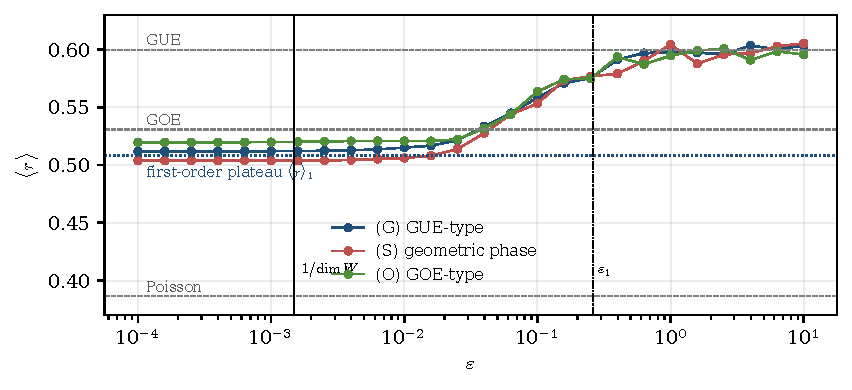
\includegraphics[width=\textwidth]{figures/fig_quantum_chaos_crossover.pdf}
\caption{The ratio statistic $\langle r\rangle$ of $U_0e^{i\varepsilon V}$ on the full space $W$ of
$Y_{168}$ ($\dim W=678$) against the perturbation strength, $\varepsilon=10^{-4},\dots,10$ ($26$ values,
$8$ samples each), for a GUE-type perturbation (G), the geometric phase perturbation (S) and a GOE-type
perturbation (O), all with $\Tr V^{2}=\dim W$. The dotted line is the first-order plateau
$\langle r\rangle_1=0.5083$ of Proposition~\ref{V3P4:prop:plateau}; the sample-to-sample scatter of the
plateau is visible below $\varepsilon\approx10^{-2}$. The solid vertical line marks the window edge
$\varepsilon=1/\dim W$, deep inside the plateau, and the dash-dotted line the first-order scale
$\varepsilon_1=0.26$ at which the mean splitting reaches the mean spacing. Saturation at the GUE value
$0.600$ occurs for $\varepsilon\gtrsim0.4$. Data of \texttt{code/v3p4\_gue\_transition.py}, drawn by
\texttt{code/make\_figures.py}.}
\label{V3P4:fig:crossover}
\end{figure}

\begin{remark}[Numerical: the window and beyond]\label{V3P4:rem:window}
\begin{enumerate}
\item[(1)] \emph{Window} $0\le\varepsilon\le1/N=1.475\cdot10^{-3}$, $21$ values, $16$ samples. For
all three families $\langle r\rangle$ is flat on the whole window and equal to the first-order
plateau computed from the same $V$:
\begin{center}\small
\begin{tabular}{lccccc}
\toprule
family & $\varepsilon=\frac1{20N}$ & $\frac1{4N}$ & $\frac1{2N}$ & $\frac1N$ & $\langle r\rangle_1$ (Prop.~\ref{V3P4:prop:plateau})\\
\midrule
(G) GUE-type & 0.5083 & 0.5084 & 0.5085 & 0.5087 & $0.5083\pm0.0030$\\
(S) geometric phase & 0.5082 & 0.5082 & 0.5083 & 0.5085 & $0.5082\pm0.0072$\\
(O) GOE-type & 0.5096 & 0.5096 & 0.5097 & 0.5099 & $0.5095\pm0.0031$\\
\bottomrule
\end{tabular}
\end{center}
At $\varepsilon=1/N$ the fraction of spacings below $0.1$ is still $0.929$, the atom itself, and the
first-order spread of a $21$-fold cluster is $0.11$ mean spacings. The real family (O) gives the
same plateau as (G) because the eigenspaces of $U_0$ are complex.
\item[(2)] \emph{Extended scan} $\varepsilon=10^{-4},\dots,10$ ($26$ values, $8$ samples;
Figure~\ref{V3P4:fig:crossover}).
$\langle r\rangle$ stays on the plateau ($0.50$--$0.52$ with $8$ samples) up to
$\varepsilon\approx10^{-2}$, rises through the GOE value near $\varepsilon\approx0.03$, and reaches
the GUE value; above $\varepsilon\approx0.4$ it fluctuates around $0.60$. The scales are
$\varepsilon_{1/2}=0.028$ (half of the spacings have opened), $\varepsilon_1=0.26$ (mean first-order
splitting $=$ mean spacing; the formula $\pi(m-1)/(2\sqrt{mN})$ with $m=21$ gives $0.263$), and
$\varepsilon_{\mathrm{sat}}=0.40$ for (G), (O) and $0.63$ for (S), i.e.\ $270$--$430$ times $1/N$;
$\langle r\rangle_{\mathrm{sat}}=0.601$, $0.600$, $0.596$.
\item[(3)] \emph{Spacing distributions} ($24$ samples, $16272$ spacings each). At $\varepsilon=1/N$
the empirical $P(s)$ is the atom plus a small continuous part; the maximum-likelihood Brody
parameter sits at the boundary $b=0$ of the family, which cannot represent an atom, and the
Kolmogorov distances to the Poisson, GOE and GUE laws are $0.91$--$0.93$. At $\varepsilon=\varepsilon_1$:
$\langle r\rangle=0.577$ and $0.580$, still $b=0$ because of the excess of small spacings. At
$\varepsilon=3$: $\langle r\rangle=0.601$ (G), $0.597$ (S), $b=1.53$ and $1.51$ (the GUE value of
the estimator, Remark~\ref{V3P4:rem:brodyfit}), Kolmogorov distance $0.005$ and $0.010$ to the GUE
surmise against $0.069$ and $0.072$ to GOE.
\end{enumerate}
So the answer to the question is negative in the window and positive outside it: on
$0<\varepsilon\le1/\dim W$ the statistic is pinned at the plateau $\langle r\rangle_1\approx0.51$
of Proposition~\ref{V3P4:prop:plateau}, and the GUE value $0.600$ is reached only for
$\varepsilon\gtrsim0.4$, where the first-order splittings exceed the mean spacing; the scale is
$\varepsilon_1\propto(m-1)/\sqrt{mN}$, not $1/N$.
\end{remark}

\begin{remark}[Scope]\label{V3P4:rem:chaosscope}
Proved: Propositions~\ref{V3P4:prop:firstorder}, \ref{V3P4:prop:noT}(i)--(iii),
\ref{V3P4:prop:symfam}, \ref{V3P4:prop:deck} except the block dimensions,
\ref{V3P4:prop:aut}(i)--(ii), \ref{V3P4:prop:equiv}, \ref{V3P4:prop:plateau}. Numerical, with the
code as the record: Tables~\ref{V3P4:tab:cross} and~\ref{V3P4:tab:sat}, Remark~\ref{V3P4:rem:window}, the block dimensions and spectra, the lifts and
their orbits, the certificate $\kappa_{1,2}(V_0)\ne0$, and the persistence of the Galois triples
under pull-back potentials. Not proved: any universality statement for the family
$U_\varepsilon$ as $n\to\infty$; the numbers here concern one complex, $Y_{168}$, and what they
establish is that on this complex the crossover scale is the first-order splitting scale, and the
symmetry class is decided by the antiunitary symmetries of the perturbed family, in the sense of
\cite{BGS84,KS97}, not by the arithmetic that produced the degeneracy.
\end{remark}


\section{Verification battery}\label{V3P4:sec:battery}

\begin{table}[ht]
\centering\scriptsize
\renewcommand{\arraystretch}{1.2}
\resizebox{\textwidth}{!}{%
\begin{tabular}{lcl}
\toprule
check & complexes & result\\
\midrule
(R) sums $q^{2}$; block-cyclic; the relations of Proposition~\ref{V3P4:prop:relations} & five covers & exact\\
(U) $W$ is $L_E^{t}$-invariant, $\|L_E^{t}f\|=\sqrt2\|f\|$; $\operatorname{rank}\Psi=3n-6$, $\dim W=4n+6$ & five covers & numeric $10^{-10}$\\
(F) $\operatorname{spec}L_E$ as in Theorem~\ref{V3P4:thm:factor}; $|\lambda|\ge\sqrt2$; Ramanujan; circle counts $(q,\sqrt q)$: & & \\
\quad $Y_{21}$ $(54,90)$, $Y_{24}$ $(63,102)$, $Y_{42}$ $(117,174)$, $Y_{84}$ $(243,342)$, $Y_{168}$ $(495,678)$ & five covers & numeric $10^{-6}$\\
(X) the $Y_{21}$ product formula at $u=1,2,3,-1,-2,5,7,-3$ & $Y_{21}$ & exact\\
(K) $\ker\Psi$ $6$-dimensional, trivial characters; $\Gamma_q$ property and disjointness from tempered $a$ ($q\le5$) & five covers & numeric\\
(D) $J-\operatorname{Inc}(\PG(d,q))$: sums $q^{d}$, $q^{d-1}$ on $\mathbf 1^{\perp}$, $(d,q)\in\{(2,2),(2,3),(3,2),(3,3),(4,2)\}$ & --- & numeric $10^{-8}$\\
(S) distinct $\lambda^{3}$ on $W$: $4,6,16,16,16$; atom $210/226$; perturbation table & $Y_{168}$ & numeric (seed 1)\\
(B) Brody $b=1$ is the GOE surmise; $b=2$ differs from GUE by $0.162$ (sup) & --- & numeric\\
\bottomrule
\end{tabular}}
\medskip
\caption{Checks run by \texttt{code/v3p4\_verify.py}. Section~\ref{V3P4:sec:chaos} is checked by
\texttt{code/v3p4\_quantum\_chaos.py} and \texttt{code/v3p4\_gue\_transition.py}.}
\label{V3P4:tab:battery}
\end{table}

\section{Scope, residue, corrections}\label{V3P4:sec:scope}

\begin{remark}[Solved, open]\label{V3P4:rem:scope}
\emph{Solved:} the local form and intertwining relations of $L_E$; the unconditional unitary
remainder, for all $d$; the lower bound $|\lambda|\ge q^{(d-1)/2}$; the factorization and the
Ramanujan equivalence for $d=2$; the exact kernel of $\Psi$; the exact polynomial for $Y_{21}$.
\emph{Open:} (a) the vertex block for $d\ge3$, which needs one operator like $Q$ for each
intermediate type; (b) an explanation of the few distinct remainder values on abelian covers;
(c) a (L)-complex with $q\ge2$ that is not Ramanujan, or a proof that none exists among
quotients of a given building; (d) any universality statement for the eigenphases of $U$ along
families.
\end{remark}

\begin{remark}[Corrections to the proposed programme]\label{V3P4:rem:corrections}
(1) The block structure of $L_E$ is cyclic in the type grading, not tridiagonal. (2) The
unconditional theorem is the unitary remainder on $W$, with $\rho=q^{(d-1)/2}$. The spectral
radius of $L_E$ away from the Perron orbit is $q$, not $q^{(d-1)/2}$, and the full
Riemann hypothesis for $\det(I-uL_E)$, in its two-circle form, is \emph{equivalent} to the
Ramanujan property (Theorem~\ref{V3P4:thm:ramanujan}). (3) Degenerate spectra have an atom at
$0$ and are not Poisson (Proposition~\ref{V3P4:prop:atom}). $\PGL_{d+1}(\F_q)$ acts on links,
not on $Y$. (4) $L_E$ is not Hermitian, so $L_E+\varepsilon V$ is not a Hamiltonian. The
natural unitary object is $U$ on $W$. A ``nonlinear'' perturbation has no spectrum; we use
linear ones. (5) Small $\varepsilon$ splits degeneracies but does not produce Wigner--Dyson
statistics (Proposition~\ref{V3P4:prop:split}); the crossover requires splittings of the order
of the mean spacing. (6) Brody's parameter is not Dyson's $\beta$: $b=2$ is not GUE
(Proposition~\ref{V3P4:prop:brody}). GOE versus GUE is decided by antiunitary symmetries
(Remark~\ref{V3P4:rem:numerics}(3)). (7) The ``unification'' is the decomposition
$\operatorname{im}\Psi\oplus W$, not an implication between Ramanujan and chaos
(Remark~\ref{V3P4:rem:unify}).
\end{remark}

\section*{Acknowledgement of provenance and caveats}

Unrefereed. The definition of Ramanujan complexes is that of \cite{LSV05}. The two-circle
characterization is in the spirit of \cite{KLW10}, and it is proved here independently. The
perturbation-theoretic and random-matrix references \cite{Kato,Brody73,Atas13,KS97,BGS84,JMRR99}
are cited for standard facts and terminology. The bibliographic data of these references
have been checked against Crossref and zbMATH.
